\documentclass[14pt]{extarticle}
% math symbols
\usepackage{sfg}


\usepackage{amssymb,amsmath}
\synctex=1
% for different compilers
\usepackage{ifpdf}
% geometry of page
\usepackage[margin=2cm]{geometry}

% if pdflatex, then
\ifpdf
\usepackage[russian]{babel}
\usepackage[utf8]{inputenc}
\usepackage[unicode]{hyperref}
\usepackage[pdftex]{graphicx}
\usepackage{cmlgc}
% if xelatex, then
\else
% math fonts
\usepackage{fouriernc}
% xelatex specific packages
\usepackage[xetex]{hyperref}
\usepackage{xltxtra}	% \XeLaTeX macro
\usepackage{xunicode}	% some extra unicode support
\defaultfontfeatures{Mapping=tex-text}
\usepackage{polyglossia}	% instead of babel in xelatex
\usepackage{indentfirst}	% 
\setdefaultlanguage{russian}
% fonts
\newfontfamily\cyrillicfont{SchoolBookC}
\newfontfamily\cyrillicfontsf{TextBookC}
\setmonofont{Consolas}
\fi

% several pictures in one figure
\usepackage{subfig}
% calc in TeX expressions
\usepackage{calc}
% nice pictures and plots
\usepackage{pgfplots,tikz,circuitikz}
% different libraries for pictures
\usetikzlibrary{%
  arrows,%
  calc,%
  patterns,%
  decorations.pathreplacing,%
  decorations.pathmorphing,%
  decorations.markings,%
  intersections,%
  decorations.text%
}

\usepackage{tkz-euclide}

\usepackage{enumitem}
\renewcommand{\theenumi}{(\asbuk{enumi})}
\renewcommand{\labelenumi}{\asbuk{enumi})}
\AddEnumerateCounter{\Asbuk}{\@Asbuk}{\CYRM}
\AddEnumerateCounter{\asbuk}{\@asbuk}{\cyrm}

\begin{document}

\section*{Задача}

\subsection*{Условие}
В правильном тетраедре с ребром 2 проводится сечение плоскостью, параллельной одной из гранией. Выразите площадь этого сечения как $f(x)$, где $x$ -- расстояние между гранью и плоскостью сечения.
\subsection*{Решение}

Заметим, что, поскольку $B_0B_1B_2 || A_0A_1A_2$, 

\begin{align*}
OA_0A_1 \sim OB_0B_1; \\
OA_1A_2 \sim OB_1B_2; \\
OA_2A_0 \sim OB_2B_0.
\end{align*}
Причем эти три подобия имеют обинаковые коэффициенты, поскольку имеют общие стороны. Обозначим этот коэфициент подобия за $\alpha$. Если $P$ и $Q$ -- середины сторон $B_0B_1$ и $A_0A_1$ соответственно, то 

\begin{equation}
OP = \alpha OQ,
\end{equation}
как медианы подобных. А значит их высоты тоже относятся в $\alpha$ раз. Тогда, поскольку $B_0B_1B_2 \sim A_0A_1A_2$ тоже с коэффициентом $\alpha$, $S_B = \alpha^2 S_A$. Известно, что высота правильного тетраедра равна $\sqrt{2/3}a = 2\sqrt{2/3}$. А значит, что $S_B={(1 - \sqrt{3/8}x)}^2 S_A = {(1 - \sqrt{3/8}x)}^2 \sqrt{3}$

\newpage
\begin{figure}[h]
	\centering
	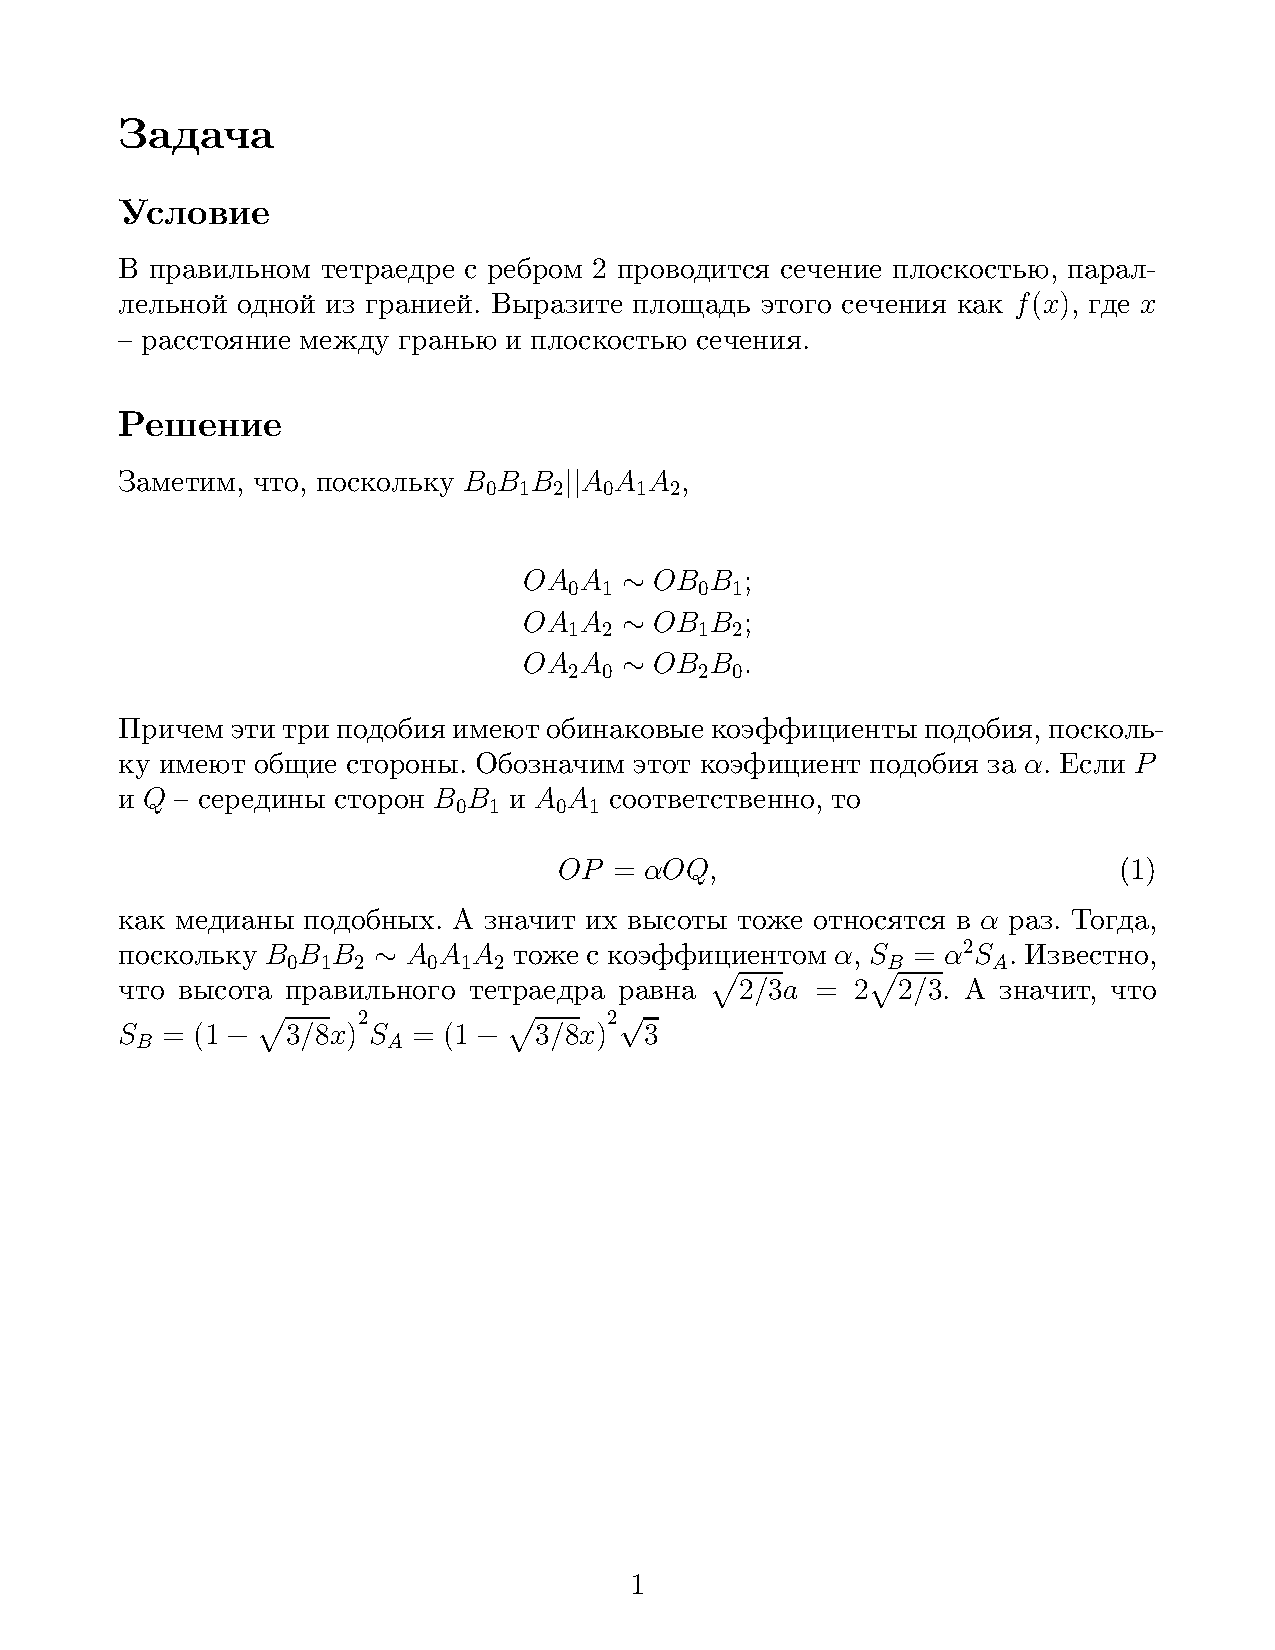
\includegraphics[width=1\textwidth]{{./12.34}.png}
\end{figure}


\end{document}